\section{15-10-2014}
\subsection{Markov Chains 1.6}

\begin{thm}
A state \(i\) is recurrent if and only if \(\sum _{n=0}^\infty p_{ii}^{(n)}=\infty .\)
\end{thm}

\begin{thm}[Example 1.6.1 The simple random walk on \(\Bbb{Z}\)]
Compute \(\sum _{n=0}^\infty p_{00}^{(n)}.\)
\end{thm}

\begin{proof}
First note that \(p_{00}^{(2n+1)}=0.\)

Any given sequence of steps of length \(2n\) from \(0\) to \(0\) occurs with probability \(p^nq^n\), there being \(n\) steps up and \(n\) steps down. And the number of such sequences is the number of ways of choosing the \(n\) steps up from \(2n\). Thus
\[
p_{00}^{(2n)}={2n\choose n}p^nq^n=\frac{(2n)!}{n!^2}(pq)^n.
\]
Remember that
\[
n! \simeq  \sqrt {2\pi n}(n/e)^n  \qquad n\rightarrow \infty .
\]
So
\begin{align*}
(2n)! &\simeq  \sqrt {4\pi n}(2n/e)^{2n}  &\qquad n\rightarrow \infty \\
n!^{2} &\simeq  {2\pi n}(n/e)^{2n}  &\qquad n\rightarrow \infty .
\end{align*}
And therefore
\begin{align*}
\frac{(2n)!}{n!^2}(pq)^n\simeq \frac{(4pq)^n}{\sqrt {\pi n}} &\qquad n\rightarrow \infty 
\end{align*}

\begin{itemize}
  \item \(p=q:\) Then \(p=q=1/2\), so \(4pq=1\). And we have
\begin{align*}
p_{00}^{(2n)}\simeq \frac{1}{\sqrt {\pi n}} &\qquad n\rightarrow \infty 
\end{align*}
which is equivalent with
\[
\forall \epsilon>0\  \exists N:n\geq N\Longrightarrow \frac{1}{\sqrt {\pi }\sqrt {n}}-\epsilon<p_{00}^{(2n)}<\frac{1}{\sqrt {\pi n}}+\epsilon.
\]
So there exists a \(N\) such that for all \(n\geq N\) we have
\[
p_{00}^{(2n)}>\frac{1}{2\sqrt n}.
\]
Therefore
\[
\sum _{n=0}^\infty p_{00}^{(n)}>\sum _{n=N}^\infty p_{00}^{(2n)}>\sum _{n=N}^\infty \frac{1}{2\sqrt n}=\infty 
\]
  \item \(p\neq q:\) Then \(4pq=r<1.\) And we have
\begin{align*}
p_{00}^{(2n)}\simeq \frac{r^n}{\sqrt {\pi n}} &\qquad n\rightarrow \infty 
\end{align*}
which is equivalent with
\[
\forall \epsilon>0\  \exists N:n\geq N\Longrightarrow \frac{r^n}{\sqrt {\pi }\sqrt {n}}-\epsilon<p_{00}^{(2n)}<\frac{r^n}{\sqrt {\pi n}}+\epsilon.
\]
So there exists a \(N\) such that for all \(n\geq N\)  we have
\[
p_{00}^{(2n)}<r^n
\]
Therefore
\[
\sum _{n=N}^\infty p_{00}^{(n)}=\sum _{n=N}^\infty p_{00}^{(2n)}<\sum _{n=N}^\infty r^n<\infty .
\]
And therefore
\[
\sum _{n=0}^\infty p_{00}^{(n)}<\infty .
\]
\end{itemize}

\end{proof}

\begin{thm}[Example 1.6.2 The simple random walk on \(\Bbb{Z}^{2}\)]
Compute \(\sum _{n=0}^\infty p_{00}^{(n)}.\)
\end{thm}

\begin{proof}
By rotating \(\Bbb{Z}^{2}\) we get that each step is like moving in one step in each of the independent, one dimensional, simple random walks. Hence
\[
p_{00}^{(2n)}\simeq \bigg(\frac{1}{\sqrt {\pi n}}\bigg)^2=\frac{1}{\pi n}
\]
which is equivalent with
\[
\forall \epsilon>0\  \exists N:n\geq N\Longrightarrow \frac{1}{\pi n}-\epsilon<p_{00}^{(2n)}<\frac{1}{\pi n}+\epsilon.
\]
So there exists a \(N\) such that for all \(n\geq N\) we have
\[
p_{00}^{(2n)}>\frac{1}{4n}.
\]
Therefore
\[
\sum _{n=0}^\infty p_{00}^{(n)}>\sum _{n=N}^\infty p_{00}^{(2n)}>\frac{1}{4}\sum _{n=N}^\infty \frac{1}{n}=\infty 
\]

\end{proof}
\subsection{Markov Chains 1.7}
\begin{defn}
We say that a measure \(\lambda =(\lambda _{i}: i\in I)\) where \(\lambda _{i}\geq 0\) is \emph{invariant} if
\[
\lambda P=\lambda .
\]
\end{defn}

\begin{thm}[Theorem 1.7.1]
Let \((X_{n})_{n\geq 0}\) be a Markov\((\lambda ,P)\) and suppose that \(\lambda \) is invariant for \(P\). Then \((X_{n+m})_{n\geq 0}\) is also Markov \((\lambda ,P)\).
\end{thm}

\begin{thm}[Theorem 1.7.2]
Let \(I\) be finite. Suppose for some \(i\in I\) that for all \(j\in J\)
\[
p_{ij}^{(n)}\rightarrow \pi _{j} \qquad n\rightarrow \infty .
\]
Then \(\pi =(\pi _{j}:j\in I)\) is an invariant distribution.
\end{thm}

\begin{prop}
Give a example of infinite state space \(I\) where Theorem 1.7.2 doesn't hold.
\end{prop}

\begin{proof}
For the random walk in \(\Bbb{Z}\) we have for all \(i,j\in I\)
\[
p_{ij}^n\rightarrow 0 \qquad n\rightarrow \infty .
\]
Note however that \((0,0,\ldots )\) is not a distrubution. As the total mass
\[
\sum _{i\in I}\lambda _{i}=0\neq 1.
\]
\end{proof}


\begin{thm}
Consider a recurrence relation of the form
\[
x_{n+1}=ax_{n}+b.
\]
The general solution is
\[
x_{n}=\begin{cases}Aa^n+b/(1-a) &a\neq 1\\ x_{n}=x_{0}+nb &a=1\end{cases}
\]
\end{thm}

\begin{thm}[Example 1.1.4]
The most general two-state chain has transition matrix of the form
\[
P= \begin{pmatrix}1-\alpha &\alpha  \\ \beta &1-\beta \end{pmatrix}.
\]
Draw the diagram, and find \(p_{11}^{(n)}.\)
\end{thm}

\begin{proof}
\begin{tikzpicture}
\SetGraphUnit{3}
\Vertices{line}{1,2}
\tikzset{EdgeStyle/.append style = {bend left}}
\Edge[label=$\beta$](2)(1)
\Edge[label=$\alpha$](1)(2)
\end{tikzpicture}

We have that
\[
P^{n+1}=P^n\begin{pmatrix}1-\alpha &\alpha  \\ \beta &1-\beta \end{pmatrix}.
\]
And therefore
\[
p_{11}^{(n+1)}=p_{11}^{(n)}(1-\alpha )+ p_{12}^{(n)}\beta .
\]
Note that we have
\[
p_{12}^{(n)}=1-p_{11}^{(n)}.
\]
So we have
\[
p_{11}^{(n+1)}=p_{11}^{(n)}(1-\alpha -\beta )+ \beta .
\]
The general solution of this recurrence relation is
\[
p_{11}^{(n)}=
\begin{cases}A(1-\alpha +\beta )^n+\alpha /(\alpha +\beta ) &(1-\alpha +\beta )\neq 1 \\
1+n\beta  &1-\alpha +\beta =1\end{cases}
\]

This reduces to:
\[
p_{11}^{(n)}=
\begin{cases}\frac{\beta }{\alpha +\beta } (1-\alpha +\beta )^n+\alpha /(\alpha +\beta ) &\alpha +\beta >0 \\
1 &\alpha =\beta =0\end{cases}
\]

\end{proof}


\begin{prop}
Consider the two-state Markov chain with transition matrix
\[
P=
\begin{pmatrix}1-\alpha &\alpha \\
\beta &1-\beta \end{pmatrix}
\]
Ignore the trivial cases \(\alpha =\beta =0\) and \(\alpha =\beta =1.\)
\end{prop}

\begin{proof}
From example 1.1.4 we have
\[
p_{11}^{(n)}=
\begin{cases}\frac{\alpha }{\alpha +\beta } (1-\alpha -\beta )^n+\beta /(\alpha +\beta ) &\alpha +\beta >0 \\
1 &\alpha =\beta =0\end{cases}
\]
In a similar we could have shown that
\[
p_{12}^{(n)}=
\begin{cases}\frac{\alpha }{\alpha +\beta } (1-\alpha -\beta )^n+\alpha /(\alpha +\beta ) &\alpha +\beta >0 \\
1 &\alpha =\beta =0\end{cases}
\]

Therefore \(p_{11}^{(n)}\rightarrow \frac{\beta }{\alpha +\beta }\) and \(p_{12}^{(n)}\rightarrow \frac{\alpha }{\alpha +\beta }\). And by theorem 1.7.2 we get that
\[
\bigg(\frac{\beta }{\alpha +\beta },\frac{\alpha }{\alpha +\beta }\bigg)
\]
is an invariant distribution.
\end{proof}

\begin{defn}
For a fixed state \(k\), consider for each \(i\) the expected time spent in \(i\) between visits to \(k\):
\[
\gamma _{i}^k=E_{k} \sum _{n=0}^{T_{k}-1}1_{\{X_{n}=i\}}
\]
\end{defn}

\begin{thm}[Theorem 1.7.5]
Let \(P\) be irreducible and recurrent. Then

\begin{enumerate}
  \item \(\gamma _{k}^k=1\)
  \item \(\gamma ^k=(\gamma _{i}^k:i\in I)\) satisfies \(\gamma ^kP=\gamma ^k\)
  \item \(0<\gamma _{i}^k<\infty \) for all \(i\in I\)
\end{enumerate}
\end{thm}


\begin{thm}[Theorem 1.7.6]
Let \(P\) be irreducible and let \(\lambda \) be an invariant measure for \(P\) with \(\lambda _{k}=1\). Then \(\lambda \geq \gamma ^k\). If in addition \(P\) is recurrent, then \(\lambda =\gamma ^k\).
\end{thm}

Recall that a state \(i\) is recurrent if
\[
\Bbb{P}_{i}(X_{n}=i \text{ for infinitely many } n)=1
\]
and we showed in Theorem 1.5.3 that this is equivalent to
\[
\Bbb{P}_{i}(T_{i}<\infty )=1.
\]

\begin{defn}
We call a recurrent state \(i\) positive recurrent if
\[
m_{i}=E_{i}(T_{i})<\infty .
\]
If a recurrent state fails to have this stronger property we call it \emph{null recurrent}.
\end{defn}

\begin{thm}[Theorem 1.7.7]
Let \(P\) be irreducible. Then the following are equivalent:

\begin{enumerate}
  \item every state is positive recurrent
  \item some state \(i\) is positive recurrent
  \item \(P\) has an invariant distribution \(\pi \)
\end{enumerate}

\end{thm}

\begin{thm}
If \(P\) has an invariant distribution \(\pi \), we have that \(m_{i}=E_{i}(T_{i})=\frac{1}{\pi _{i}}\) for all \(i\).
\end{thm}

\begin{thm}[Example 1.7.8]
Show that the simple symmetric random walk on \(\Bbb{Z}\) is null recurrent.
\end{thm}

\begin{proof}
The simple symmetric random walk on \(\Bbb{Z}\) is irreducible and, by example 1.6.1, it also recurrent.  Remember that
\[
(\pi P)_{j}=\sum _{i\in I}\pi _{i}p_{ij}
\]
and this equals to
\[
\sum _{i\in I}\pi _{i}p_{ij}=1/2 \pi _{j-1}+1/2\pi _{j+1}.
\]
So
\[
\pi _{i}=\tfrac{1}{2}\pi _{i-1}+\tfrac{1}{2}\pi _{i+1}.
\]
We get the equation
\[
x^2-2x+1=0.
\]
And so we have
\[
\alpha =\beta =1.
\]
And so the general solutions is
\[
\pi _{i}=A+iB.
\]
and the total mass is then
\[
\sum _{i}\pi _{i}=A\sum _{i}1+B\sum _{i}i=B\infty .
\]
So whatever \(A,B\) we choose, we never get the total mass to be zero. So there doesn't exists a invariant distribution, and by Theorem 1.7.7 we have that all states must be null recurrent.
\end{proof}
\newpage
\begin{thm}[Example 1.7.9]
Show that the existence of an invariant measure does not guarantee recurrence.
\end{thm}

\begin{proof}
The simple symmetric random walk on \(\Bbb{Z}^{3}\) has an invariant measure. Consider:
\[
(\pi P)_{j}=\sum _{i\in I}\pi _{i}p_{ij}=1/4(\pi _{a}+\pi _{b}+\pi _{c}+\pi _{d})
\]
So if we set \(\pi =(1,1,1,\ldots )\). Then \(\pi \) is invariant. But \(\Bbb{Z}^{3}\) is also transient.
\end{proof}

\begin{thm}[Example 1.7.10]
Consider the asymmetric random walk on \(\Bbb{Z}\) with transition probabilities
\(p_{i,i-1}=q<p=p_{i,i+1}\). Show that the walk is null recurrent.
\end{thm}

\begin{proof}
We have
\begin{align*}
\pi _{j}=(\pi P)_{j}&=\sum _{i\in I}\pi _{i}p_{ij}=\pi _{j-1}p_{j-1,j}+\pi _{j+1}p_{j+1,j} \\
&=\pi _{j-1}p+\pi _{j+1}q
\end{align*}
This is a recurrence relation and we have the equation
\begin{gather*}
qx^2-x+p=0  \\
D=\sqrt {1-4(1-p)p}=\sqrt {1-4p+4p^2}=1-2p \\
\alpha =\frac{-1+1-2p}{-2p}=1 \qquad \beta =\frac{-2+2p}{-2p}=\frac{1-p}{p}=\frac{q}{p}
\end{gather*}
So we have the general solution:
\[
\pi _{j}=A\alpha ^j+B\beta ^j=A+B\Big(\frac{p}{q}\Big)^i.
\]
And the total mass is therefore
\[
\sum _{j=0}^\infty \pi _{j}=\sum _{j=0}^\infty A+B\Big(\frac{p}{q}\Big)^i=B\infty .
\]

So whatever \(A,B\) we choose, we never get the total mass to be zero. So there doesn't exists a invariant distribution, and by Theorem 1.7.7 we have that all states must be null recurrent.

\end{proof}

\begin{thm}[Example 1.7.11]
Consider a success-run chain on \(\Bbb{Z}^+\), whose transition probabilities given by
\[
p_{i,i+1}=p_{i} \qquad p_{i0}=q_{i}=1-p_{i}.
\]
And where
\[
p=\prod _{i=0}^\infty p_{i}>0.
\]
Show that every state is transient.
\end{thm}

\begin{proof}
We have
\begin{align*}
\pi _{j}=(\pi P)_{j}&=\sum _{i\in I}\pi _{i}p_{ij} \\
&=\pi _{j-1}p_{j-1}\\
&=\pi _{0}\prod _{i=0}^{j-1}p_{i}
\end{align*}
and
\begin{align*}
\pi _{0}&=\sum _{i=0}^\infty \pi _{i}p_{i0}\\
&=\sum _{i=0}^\infty (1-p_{i})\pi _{i} \\
&=\pi _{0}\sum _{i=0}^\infty (1-p_{i})\prod _{j=0}^{i-1}p_{j} \\
&=\pi _{0}\sum _{i=0}^\infty \prod _{j=0}^{i-1}p_{j}-\prod _{j=0}^{i}p_{j} \\
&=\pi _{0}(1-\prod _{j=0}^{\infty }p_{j}).
\end{align*}
The last equality need some thinking, but notice that it's a telescoping sum. Define

$$a_i := \prod_{j=0}^{i-1} p_j,$$

the sum is

$$\sum_{i=0}^\infty (a_i - a_{i+1}) = a_0 - \lim_{k\to\infty} a_k= 1-\prod _{j=0}^{\infty }p_{j}$$

The equation 
\[\pi _{0}=\pi _{0}(1-\prod _{j=0}^{\infty }p_{j})\]
forces \(\pi _{0}\) to be \(0\). And therefore all \(\pi _{i}\) are zero. So there is no invariant distribution and we have that \(P\) is transient by theorem 1.7.7.
\end{proof}


